%
% $RCSfile: software_architecture.tex,v $
%
% Copyright (C) 2002-2008. Christian Heller.
%
% Permission is granted to copy, distribute and/or modify this document
% under the terms of the GNU Free Documentation License, Version 1.1 or
% any later version published by the Free Software Foundation; with no
% Invariant Sections, with no Front-Cover Texts and with no Back-Cover
% Texts. A copy of the license is included in the section entitled
% "GNU Free Documentation License".
%
% http://www.cybop.net
% - Cybernetics Oriented Programming -
%
% http://www.resmedicinae.org
% - Information in Medicine -
%
% Version: $Revision: 1.1 $ $Date: 2008-08-19 20:41:08 $ $Author: christian $
% Authors: Christian Heller <christian.heller@tuxtax.de>
%

\section{Software Architecture}
\label{software_architecture_heading}
\index{Software Architecture}
\index{Architecture Views}
\index{Four Views Model}
\index{Conceptual View}
\index{Module View}
\index{Code View}
\index{Execution View}
\index{4+1 View Model of Architecture}
\index{Rational Unified Process}
\index{RUP}
\index{Logical View}
\index{Design View}
\index{Development View}
\index{Implementation View}
\index{Physical View}
\index{Deployment View}
\index{Process View}
\index{Scenarios}
\index{Use Case +1 View}
\index{Architecture Description Languages}
\index{ADL}

As was shown in the previous sections, a software engineering process covers a
whole spectrum of activities and abstractions. Several models were created to gain
an \emph{overall} view on the resulting system architectures, across the single
software development phases. The so-called \emph{Architecture Views} that these
models provide represent \textit{a whole system from the perspective of a related
set of concerns}, as \cite{ieee1471-2000} states. Two examples are shown following.

\begin{figure}[ht]
    \begin{center}
        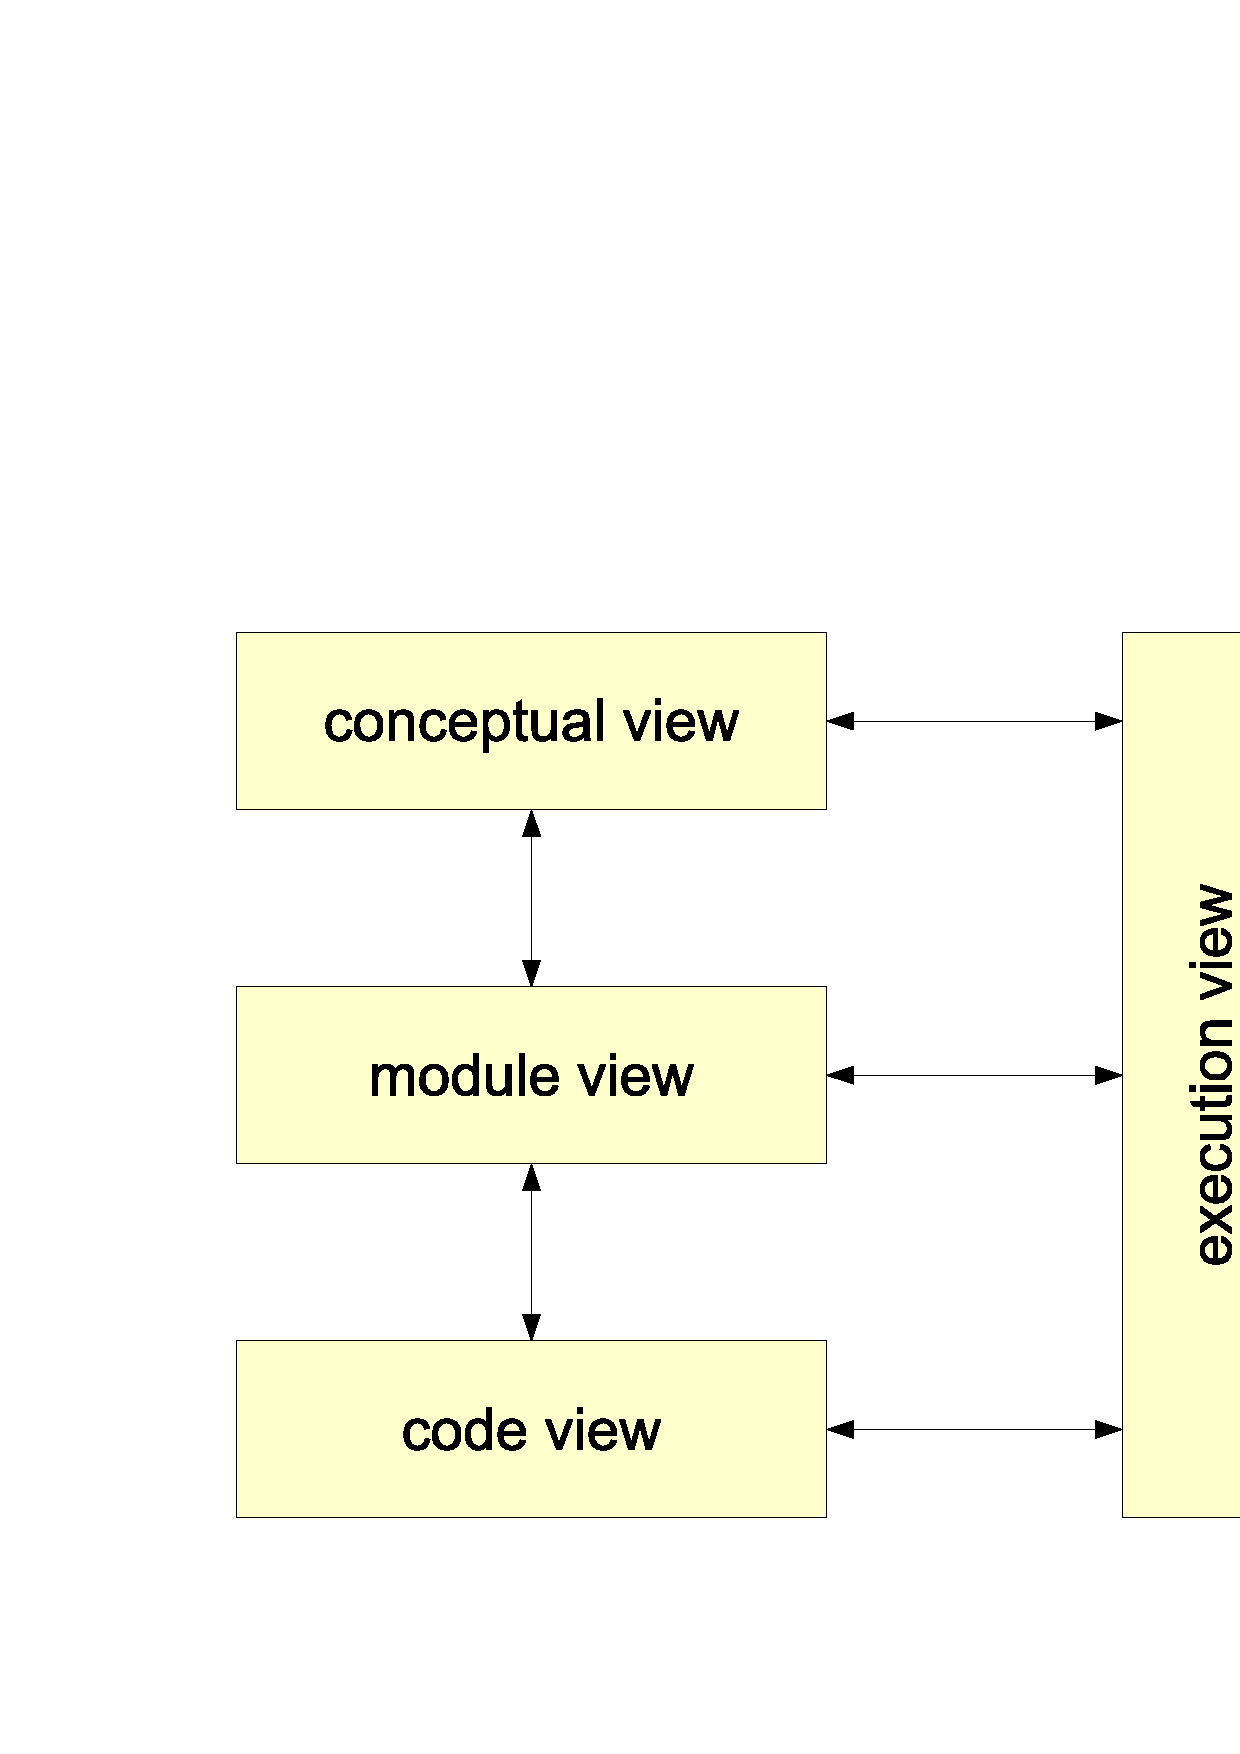
\includegraphics[scale=0.3,angle=-90]{graphic/fourviews.pdf}
        \caption{Four Views Model \cite{hofmeister}}
        \label{fourviews_figure}
    \end{center}
\end{figure}

The \emph{Four Views} model (figure \ref{fourviews_figure}) proposed by
\cite{hofmeister} is best suitable for representing architectures of systems that
are implemented in a procedural programming language. It contains four different
views that serve the following purposes:

\begin{itemize}
    \item[-] \emph{Conceptual View:} describe the major design elements of a
        system and the relations between them
    \item[-] \emph{Module View:} represent the decomposition of a system into
        modules that are grouped in layers
    \item[-] \emph{Code View:} organise source code into object code, libraries
        and binaries, and into corresponding version files and directories
    \item[-] \emph{Execution View:} map software to hardware and distribute
        software components
\end{itemize}

\begin{figure}[ht]
    \begin{center}
        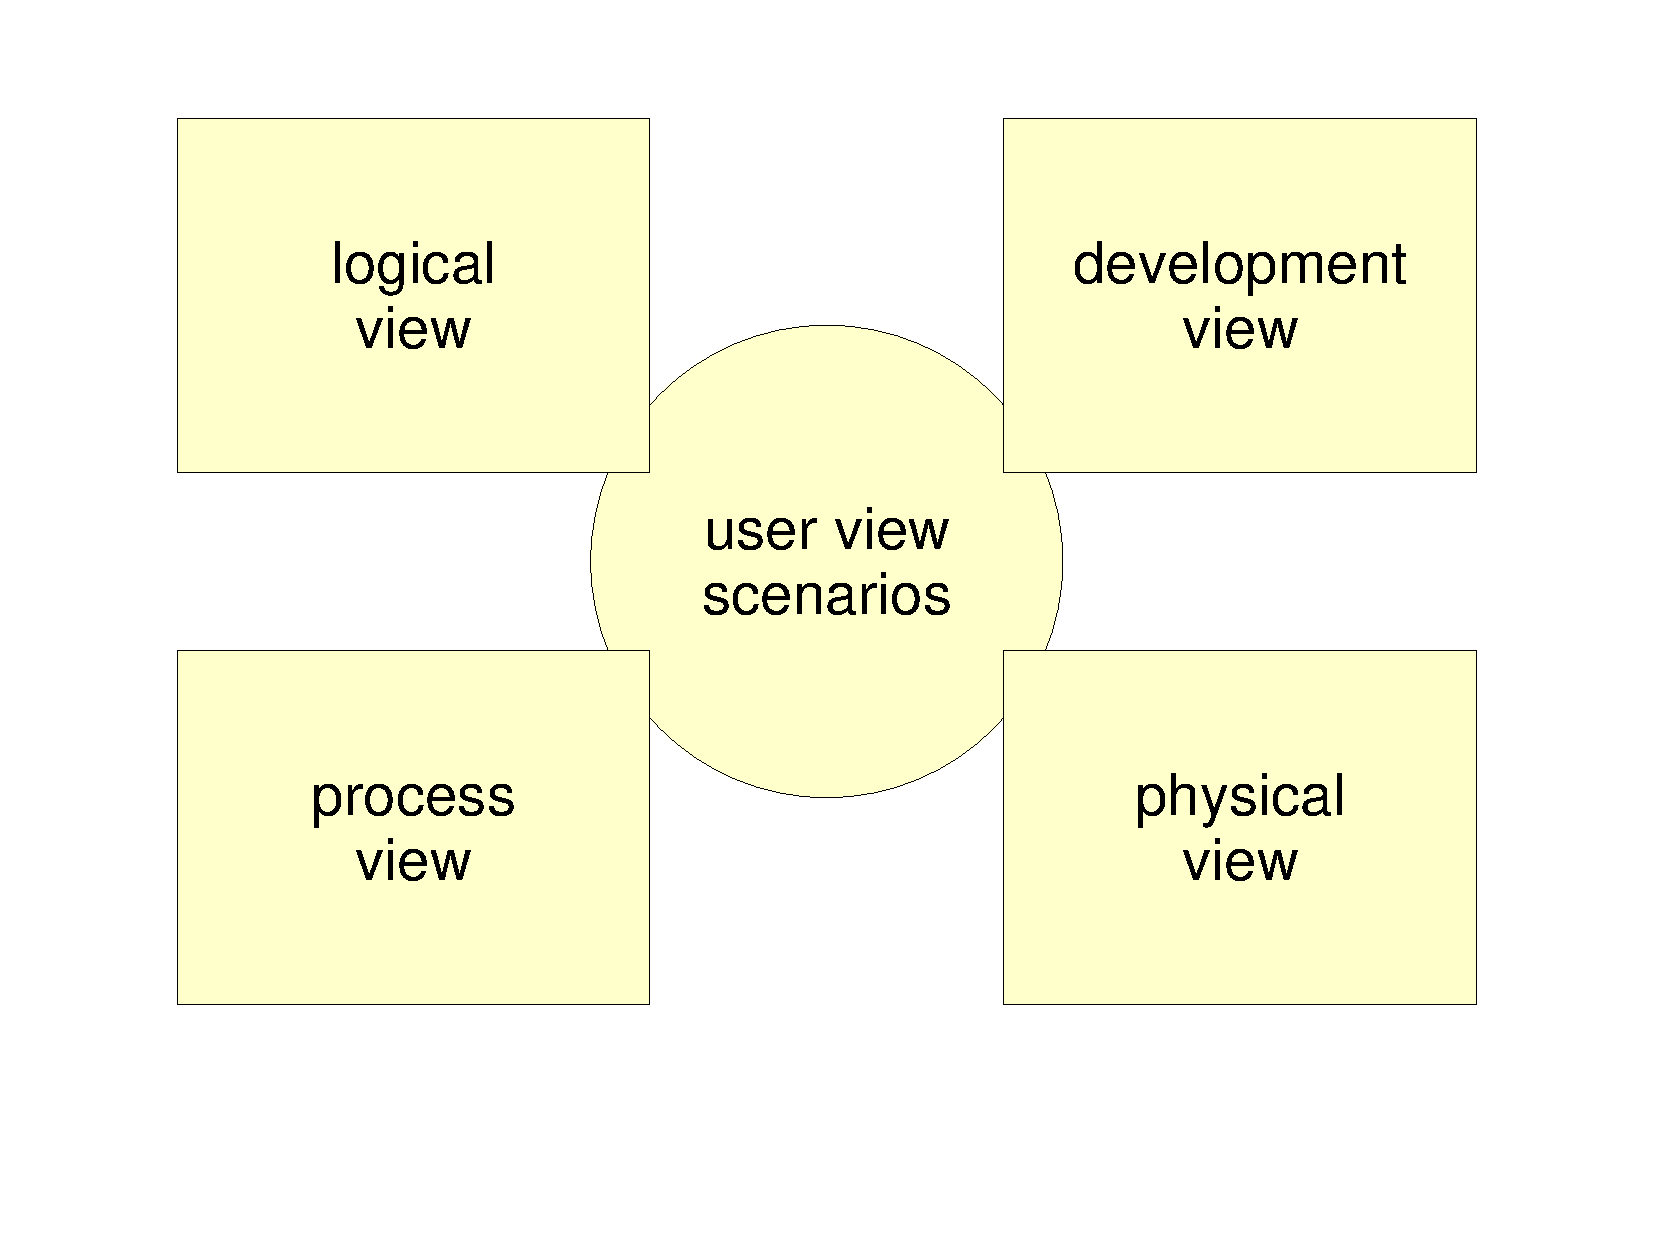
\includegraphics[scale=0.3,angle=-90]{graphic/4+1view.pdf}
        \caption{The 4+1 View Model of Architecture \cite{kruchten}}
        \label{4+1view_figure}
    \end{center}
\end{figure}

Architectures of systems that are implemented in an object-oriented way are better
represented by the \emph{4+1 View} model (figure \ref{4+1view_figure}), proposed by
\cite{kruchten} and embraced as part of the \emph{Rational Unified Process} (RUP)
\cite{rup}. It separates static and dynamic aspects and consists of five different
views, with the following purposes:

\begin{itemize}
    \item[-] \emph{Logical (Design) View:} map required system functionality to
        architecture elements
    \item[-] \emph{Development (Implementation) View:} focus on the actual
        software module organisation
    \item[-] \emph{Physical (Deployment) View:} assign software elements to
        concrete hardware nodes
    \item[-] \emph{Process View:} describe dynamic runtime behavior of the
        executed system
    \item[-] \emph{Scenarios (Use Case +1 View):} collect domain knowledge, from
        a user's view, and use them to validate and unify the other four views
\end{itemize}

Many other architecture modelling approaches like for instance the
\emph{Architecture Description Languages} (ADL), some representatives of which
are described in \cite{garlan, clements}, exist but are outside the scope of
this work and not elaborated further here, because the following two chapters
were created according to the \emph{4+1 View Model of Architecture}. Two
simplifications are made, however: The \emph{Physical-} also includes the
\emph{Process View} (chapter \ref{physical_architecture_heading}), because
processes are considered as communicating systems running on physical machines,
and the \emph{Logical-} also contains the \emph{Development View} (chapter
\ref{logical_architecture_heading}), because logical models represent
abstractions at different stages of software development. \emph{Scenarios} are
not considered since they belong to requirements engineering whose techniques
are not a topic of this work.
